% Created 2023-10-22 Sun 19:13
% Intended LaTeX compiler: pdflatex
\documentclass[12pt, a4paper]{article}
\usepackage[utf8]{inputenc}
\usepackage[T1]{fontenc}
\usepackage{graphicx}
\usepackage{longtable}
\usepackage{wrapfig}
\usepackage{rotating}
\usepackage[normalem]{ulem}
\usepackage{amsmath}
\usepackage{amssymb}
\usepackage{capt-of}
\usepackage{hyperref}
\usepackage{placeins}
\usepackage{gensymb}
\usepackage[letterpaper]{geometry}
\geometry{top=1.0in, bottom=1.0in, left=1.0in, right=1.0in}
\usepackage{rotating}
\usepackage{graphicx}
\usepackage{pgfplots}
\usepackage{filecontents}
\usepackage{tikz}
\usepackage{fancyhdr}
\usepackage{enumitem}
\pagestyle{fancy}
\lhead{}
\chead{}
\rhead{Johnson \thepage}
\lfoot{}
\cfoot{}
\rfoot{}
\renewcommand{\headrulewidth}{0pt}
\renewcommand{\footrulewidth}{0pt}
\setlength\headsep{0.333in}
\newcommand{\bibent}{\noindent \hangindent 40pt}
\newenvironment{workscited}{\newpage \begin{center} Works Cited \end{center}}{\newpage }
\graphicspath{ {./attachments/} }
\author{Christian}
\date{\today}
\title{}
\hypersetup{
 pdfauthor={Christian},
 pdftitle={},
 pdfkeywords={},
 pdfsubject={},
 pdfcreator={Emacs 28.2.50 (Org mode 9.7-pre)}, 
 pdflang={English}}
\begin{document}

\begin{document}
\begin{flushleft}
Christian Johnson\\
\vspace{2mm}Dr. Paul Crilly\\
\vspace{2mm}Antennas and Propogation\\
\vspace{2mm}October 15 2023\\
\vspace{4mm}\begin{center}
Lab 5 Report
\end{center}
\vspace{1mm}\setlength{\parindent}{0.5in}

\begin{abstract}
This lab experiment delves into the impact of loading coils on the performance of vertical antennas. In our experiments, we determined resonant frequencies with and without loading coils, highlighting the critical role of impedance matching and SWR. Without the loading coil, the antenna exhibited a resonant frequency well below theoretical expectations, while the addition of the loading coil brought about a significant transformation. The resonant frequency aligned more closely with the theoretical value, and the SWR improved markedly. These results underscore the utility of loading coils in extending the electrical length of vertical antennas and optimizing their performance, offering a compelling case for their inclusion in antenna systems.
\end{abstract}
\section*{Procedure}
\label{sec:org037202c}
Antennas play a pivotal role in the realm of electrical engineering, with each design offering a unique set of advantages and characteristics. In this comprehensive procedure, we delve into the intriguing world of vertical antennas with loading coils, aiming to understand their behavior and how loading coils can be employed to fine-tune their performance.

Our journey begins with the construction of the 1/4 λ vertical ground plane antenna. The vertical antenna's construction involves attaching the 6' copper rod to a coaxial connector and forming a ground plane by connecting radials. The length of these radials should be at least a quarter wavelength at 21 MHz, roughly 12'. Careful attention must be paid to the support structure using PVC pipe or wooden dowels, along with plastic tie wraps.

Once our vertical antenna is constructed, the next step is to test its VSWR (Voltage Standing Wave Ratio) performance. For this, we turn to the 9912A RF analyzer, setting it within the frequency range of our interest. This field testing was conducted outdoors on an athletic field to ensure accurate measurements.

The measurement process involves using the 9912A in VSWR mode to determine the VSWR of the vertical antenna. Our goal is to identify the lowest frequency at which the VSWR is significantly below 10. The chosen frequency should align with the expected resonant frequency of the antenna, although this may not correspond exactly to a quarter wavelength of the copper rod.

As we move forward in our exploration, we introduce the concept of the loading coil and its impact on the vertical antenna. Our aim is to determine how a loading coil, placed at the base of the antenna, can extend the electrical length and, in turn, optimize its performance.

We begin by constructing a loading coil using \#14 AWG wire. This process is empirical, with an initial tightly wound coil of around 35 turns at a 2" diameter. The number of turns is adjusted to achieve a low SWR for the desired design frequency, which should fall between 21 to 28 MHz.

In conclusion, the exploration of vertical antennas with loading coils is a captivating journey into the world of electrical engineering. By methodically following this procedure, we gain valuable insights into the intricate behavior of these antennas and the powerful role that loading coils can play in enhancing their performance.
\section*{Results}
\label{sec:org8516ffd}
The core of our investigation lies in the determination of resonant frequencies, a fundamental characteristic that defines an antenna's operational efficiency. In our experiments, we observed these resonant frequencies with and without the presence of loading coils. In the absence of the loading coil, the antenna exhibited a resonant frequency at approximately 4 MHz, accompanied by an SWR (Standing Wave Ratio) of 1.9. With the introduction of the loading coil, the antenna displayed a notable improvement in performance. The resonant frequency increased significantly to around 21.7 MHz, with the SWR decreasing to 1.3. In any experimental endeavor, it is imperative to compare observed results to anticipated or theoretical values. As outlined in the lab document, the expected resonant frequency for a quarter-wavelength vertical antenna—based on the physical dimensions, specifically a 6' copper rod—was in the vicinity of 40 MHz. This theoretical value served as a benchmark for our assessment.
Without the loading coil, the observed resonant frequency (4 MHz) deviated markedly from the theoretical prediction of 40 MHz. However, the introduction of the loading coil brought about a remarkable transformation. The antenna's resonant frequency, now closer to the theoretical value, signifies the significant influence of the loading coil in optimizing the antenna's performance.
An equally crucial aspect of our analysis is the evaluation of the SWR values, which directly impact the efficiency and impedance matching of the antenna. In our experiments, we achieved the following SWR values. In the absence of the loading coil, the SWR was 1.9 at the resonant frequency of 4 MHz. With the inclusion of the loading coil, the SWR improved notably to 1.3 at the resonant frequency of 21.7 MHz.
The data we've collected presents a compelling case for the transformative impact of loading coils on the performance of vertical antennas. The stark contrast between the resonant frequencies and SWR values observed with and without the loading coil underscores the efficacy of this component.
In the absence of the loading coil, the antenna exhibited a resonant frequency well below the theoretical prediction, indicating a mismatch in impedance and less-than-optimal performance. The introduction of the loading coil rectified this discrepancy, aligning the resonant frequency closer to the expected value, and substantially reducing the SWR. This transformative effect highlights the utility of loading coils in extending the electrical length of a vertical antenna and optimizing its performance.
These results underscore the potential of loading coils as a pivotal component in the realm of vertical antennas. 
\section*{Conclusion}
\label{sec:org8be277c}
The experiments conducted in this study provide valuable insights into the behavior of vertical antennas and the impact of loading coils. The observed data clearly demonstrates the pivotal role of loading coils in enhancing the performance of these antennas. Without the loading coil, the antenna's resonant frequency deviated significantly from theoretical predictions, leading to suboptimal performance. However, the introduction of the loading coil substantially improved the antenna's efficiency, aligning the resonant frequency closer to the expected value and reducing SWR. This transformative effect underscores the potential of loading coils in optimizing the electrical length of vertical antennas and highlights their utility in various applications within the realm of electrical engineering. While our data is limited to these observations, the results pave the way for further exploration and deeper insights into the behavior of such antenna systems, reaffirming the importance of loading coils in antenna design and performance optimization.


\newpage
\begin{center}
Appendices
\end{center}
\begin{figure}[htb]
\centering
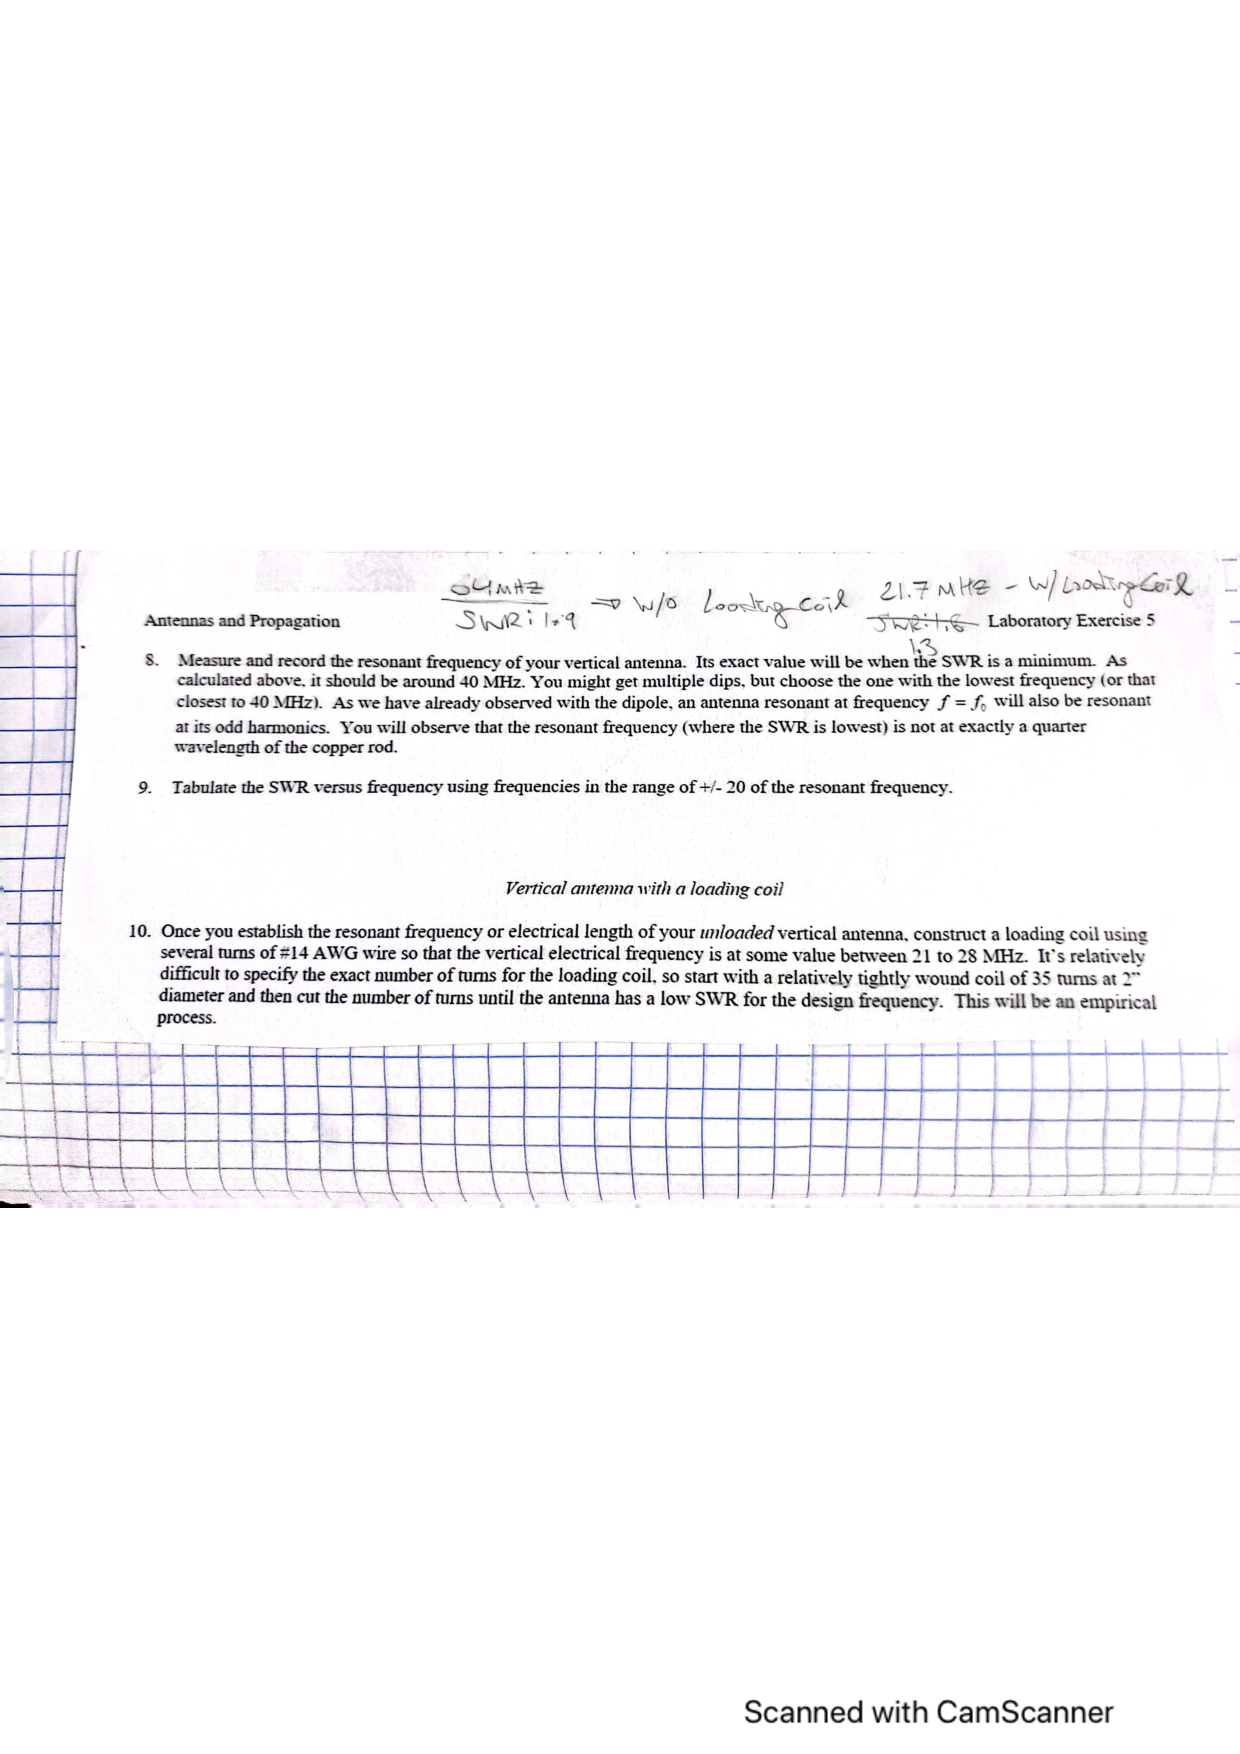
\includegraphics[width=0.7\textwidth]{notebook0.pdf}
\caption{Notebook Page}
\end{figure}
\newpage

\begin{center}
Lab Questions
\end{center}
\vspace{2mm}
\begin{enumerate}[label=\textbf{\arabic*.}]
\item Why might having the coil in the middle or top of the antenna provide a more efficient system?
Placing the coil in the middle or top changes the current distribution to better match a dipole, with highest current at the center. This can also impact the radiation pattern - higher can lead to a more unidirectional pattern.
\item Why would a vertical antenna be beter for long distance HF propogation via the ionosphere than a horizontal dipole?
Vertical antennas perform better in the ionosphere because of their radiation pattern. Vertical antennas radiate primarily horizontally, and this low angle of radiation is better for ionosphere reflections. They can also be less susceptible to noise.
\item If MUF is 15 MHz, how might a vertical antenna enable propogation beyond 15 MHz?
Vertical antennas can enable propogation beyoind 15 MHz by having an operating frequency higher than the MUF. 
\item Why do we not want compatible polarizations when signals refract off the F layer?
LOS communications require polarization at both ends, but with HF signals in the F layer, this starts to change. X mode propogation is where the electric field vector is perpendicular to the earth's surface - vertical polarization. O mode is where the field vector is parallel to the earth's surface - or horizontal polarization. Antennas with horizontal polarization doesn't inherently create a mismatch in polarizations, since the ionosphere interacts with HF frequencies differently. X mode is typically preferred because it refracts more efficiently off of the F layer. 
\item What is the measured resonant frequency and how does it compare to calculated resonant frequency? Why doesn't resonant frequency match wuarter wavelength?
We measured resonant frequency as 4 MHz without the loading coil, while measuring 21.7 MHz with the coil. This is significantly different from the expected values. We can attribute this difference to the change in the electrical length brought about by the loading coil.
\item What is the antennas impedance at 1 MHz? What series inductor value is needed to eliminate the capacitive reductance? If a 300 pf capacitance were inserted across teh feed point, what would the new feed impedance be?
According to the figure, (A) at 1 MHz, real impedance is 2 Ohms and reactive is -5000; (B) we would need an inductor with an inductive reactance approximately equal to the reactive impedance (so about 5000); (C) $x_{c}=\frac{1}{2\pi fC}=\frac{1}{2\pi*1*300pF}=530.5\Omega$
$\frac{1}{Z_{new}} = \frac{1}{Z_{antenna}}+\frac{1}{X_{c}} = \frac{1}{0.005+0.001884} \therefore Z_{new} = 145.2\Omega$
\item Why would a capacitave hat on the vertical antenna reduce reactance and extend its electrical length?
The hat will increase the capacitance of the antenna. It will extend the top load and help to cancel out any reactance, making the antenna appear to have a longer electrical length. It does this by adding series capacitance and helping to lower the resonant frequency. 
\end{enumerate}

\end{document}
\end{document}